\documentclass[12pt,a4paper,oneside]{article}
\usepackage[utf8]{vietnam}
\usepackage{amsmath}
\usepackage{amsfonts}
\usepackage{amssymb}
\usepackage{graphicx}
\usepackage[left=2cm,right=2cm,top=2cm,bottom=2cm]{geometry}
\usepackage{array}
\usepackage{fancyhdr}
\pagestyle{fancy}
\renewcommand\thesection{\Roman{section}.}
\renewcommand\thesubsection{\arabic{subsection}.}
\fancyhf{}
\rhead{{\large \textbf{Group 2}}}
\lhead{Hoàng Quốc Bảo - 20194484\\Vũ Minh Hải - 20194550}
\rfoot{Trang \thepage}

\usepackage{listings}
\usepackage{tcolorbox}
\usepackage{color} % tô màu cho code
\definecolor{dkgreen}{rgb}{0,0.6,0}
\definecolor{gray}{rgb}{0.5,0.5,0.5}
\definecolor{code}{rgb}{0.8,0.8,0.8}
\definecolor{mauve}{rgb}{0.58,0,0.82}
\lstset{frame=tb,
  language=[x86masm]Assembler,
  aboveskip=3mm,
  belowskip=3mm,
  showstringspaces=false,
  columns=flexible,
  basicstyle={\small\ttfamily},
  backgroundcolor=\color{gray!20!white},
  numbers=none,
  breaklines=true,
  breakatwhitespace=true,
  tabsize=3
}

\begin{document}
\section*{{\huge Exercise 2:}}
\subsection*{Đề bài:}
Find all prime numbers (such as 2, 3, 5, 7, etc) in a range from the integer N to the integer M. N, M is entered from the keyboard.
\subsection*{Lưu đồ thuật toán:}
\begin{center}
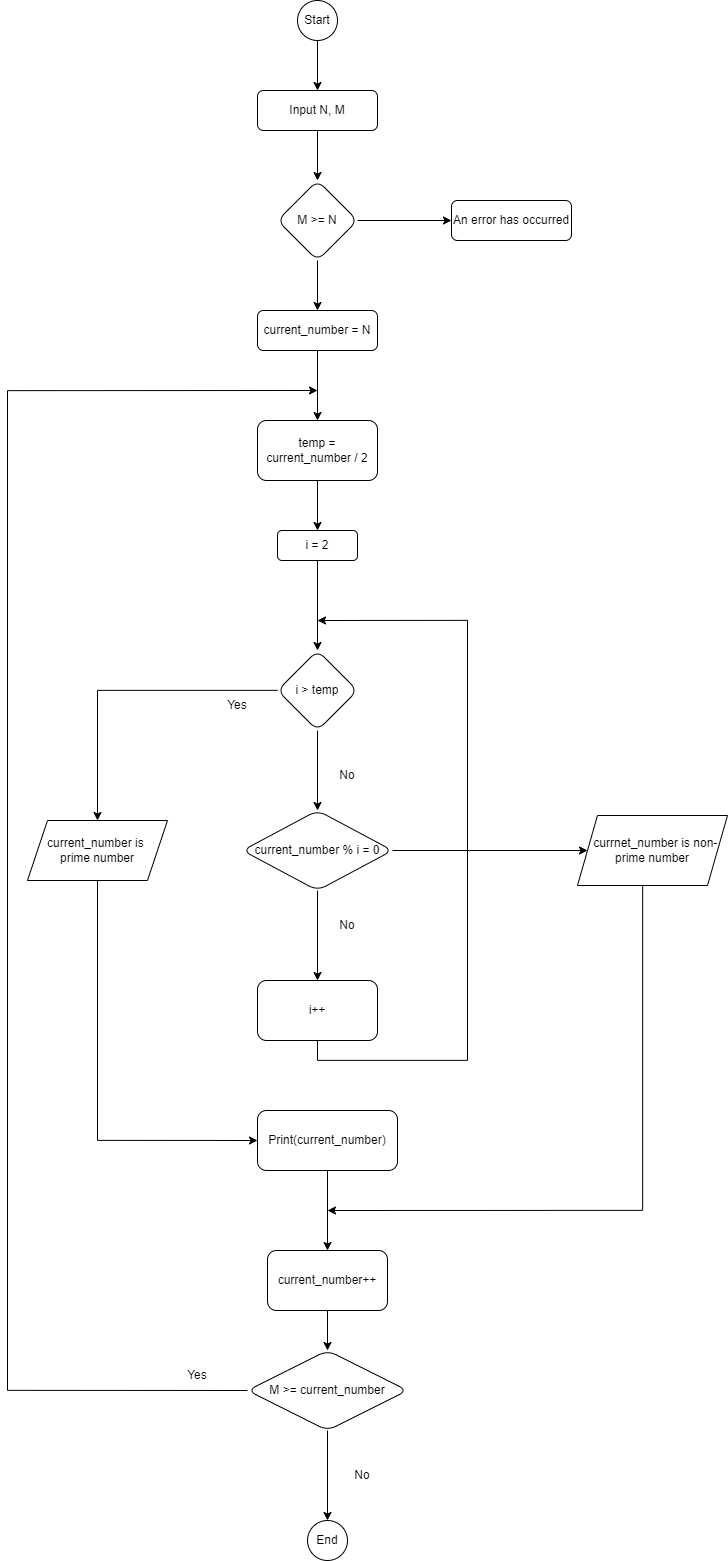
\includegraphics[scale=0.37]{b2}
\end{center}
\subsection*{Mã nguồn:}

\begin{center}
\begin{lstlisting}
.data
Message1: .asciiz "Input the integer N:"
Message2: .asciiz "Input the integer M:"
Message3: .asciiz "An error has occurred (M < N)"

.text

check\_inputN:	
		addi $v0, $zero, 51		# Read input N
		la $a0, Message1
		syscall
		bne $a1, 0, check\_inputN	# if $a1 != 0: an error has occurred, branch to check\_inputN
		nop
		add $s0, $zero, $a0		# Store N in $s0

check\_inputM:
		addi $v0, $zero, 51		# Read input N
		la $a0, Message2
		syscall
		bne $a1, 0, check\_inputM	# if $a1 != 0: an error has occurred, branch to check\_inputM
		nop
		add $s1, $zero, $a0		# Store M in $s1

		slt $t0, $s1, $s0		# if M < N: an error has occurred, end program
		bne $t0, 1, ok
		nop
		addi $v0, $zero, 55
		la $a0, Message3
		syscall
		j done
		nop

ok:
		add $s2, $zero, $s0		# initialize current\_number = N
		slti $t0, $s2, 2		# if current\_number < 2 then current\_number = 2
		bne $t0, 1, main\_loop	
		nop	
		addi $s2, $zero, 2		# current\_number = 2
main\_loop:		
		slt $t0, $s1, $s2		# if current\_number > M then end program
		beq $t0, 1, done
		nop			
		jal isprime
		nop
		bne $t1, 1, continue		# continue if current\_number is non-prime
		nop
		jal print\_number		# if current\_number is prime number, then print it
		nop
continue:	
		addi $s2, $s2, 1		# current\_number = current\_number + 1		
		j main\_loop
		

	
isprime:
push:		
		addi $sp, $sp, -12		# adjust the stack pointer
		sw $s0, 8($sp)			# store $s0 (N)
		sw $s1, 4($sp)			# store $s1 (M)
		sw $s2, 0($sp)			# store $s2 (current\_number)

work:		
		addi $t1, $zero, 1		# initialize return value = 1 (if $t1 = 1 then current\_number is prime number)
		srl $s1, $s2, 1			# temp = current\_number/2
		addi $s3, $zero, 2		# initialize i = 2
loop:
		slt $t0, $s1, $s3		# if i > temp then end procedure
		beq $t0, 1, pop 
		nop
		
		div $s4, $s2, $s3		# $s4 = current\_number / i 
		mul $s4, $s4, $s3		# $s4 = $s4 * i
		slt $t0, $s4, $s2		# if ($s4 = current\_number) then current\_number is divisible by i 
		bne $t0, 1, noprime		# curent\_number is non-prime number
		nop
		addi $s3, $s3, 1		# i = i+1
		j loop
		nop
noprime:
		add $t1, $zero, $zero		# set $v0 = 0, end procedure	
pop:		
		lw $s2, 0($sp)			# restore $s2 (current\_number)
		lw $s1, 4($sp)			# restore $s1 (M)
		lw $s0, 8($sp)			# restore $s0 (N)
		addi $sp, $sp, 12		# adjust the stack pointer
		jr $ra				# end procedure


print\_number:
		addi $v0, $zero, 1		
		add $a0, $zero, $s2
		syscall
		addi $v0, $zero, 11
		li $a0, ' '
		syscall
		jr $ra

done:

\end{lstlisting}
\end{center}
\subsection*{Giải thích phần chương trình chính:}
\begin{itemize}
	\item Khởi tạo giá trị: \\
	- Chúng ta khởi tạo 3 Message như hình dưới.
	\begin{center}
	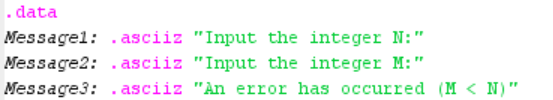
\includegraphics[scale=1]{0}
	\end{center}
	\item Nhập giá trị input N, M
	\begin{center}
	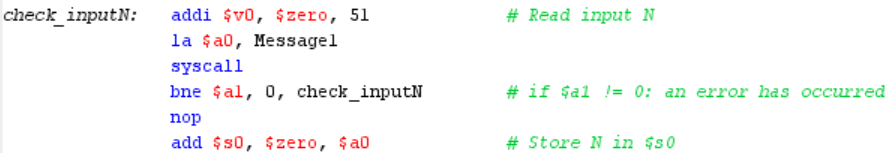
\includegraphics[scale=1]{1}
	\end{center}
	- Nếu giá trị của N nhập vào không phải là số tự nhiên, thì thanh ghi \$a1 $\neq$ 0. Lệnh bne sẽ quay lại nhãn \textit{check\_inputN} và bắt người dùng nhập lại N đến khi thoả mãn. \\\textit{(Tương tự với M)}. Giá trị của N được lưu ở thanh ghi \$s0, M ở \$s1.
	\\- \textit{Thực hiện chương trình:}\\Nhập vào giá trị N = 44, M = 84. Kết quả thực hiện:
	\begin{center}
	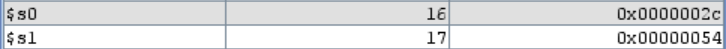
\includegraphics[scale=1]{3}
	\end{center}
	\item Kiểm tra điều kiện của M và N
	\begin{center}
	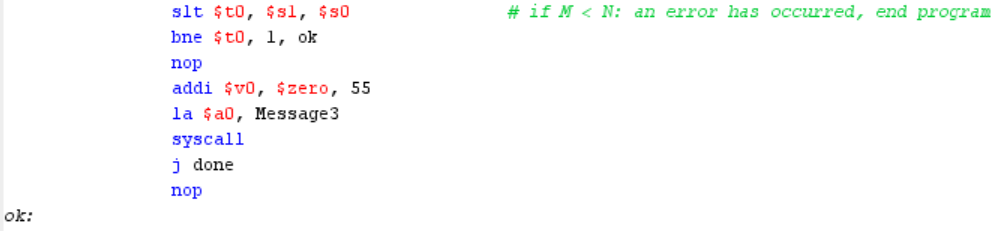
\includegraphics[scale=0.9]{2}
	\end{center}
	- Lệnh \textit{slt} và \textit{bne} kiểm tra giá trị của M và N, nếu người dùng nhập vào M < N thì câu lệnh \textit{syscall} sẽ gọi đến chức năng \textbf{MessageDialog} \textit{(\$v0 = 55)} để thông báo lỗi (Message3: "An error has occurred (M < N)") và nhảy đến nhãn done, kết thúc chương trình.\\ - Nếu người dùng nhập vào M $\geq$ N thì lệnh \textit{bne} sẽ nhảy đến nhãn \textit{ok}, chương trình tiếp tục được thực hiện.
	\\- \textit{Thực hiện chương trình:} \\Giá trị của thanh ghi \$t0 = 0. Chứng tỏ M $\geq$ N, chương trình nhảy đến nhãn \textit{ok}.
	\begin{center}
	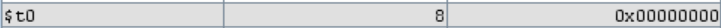
\includegraphics[scale=1]{4}
	\end{center}
	\item Khởi tạo giá trị \textit{current\_number}
	\begin{center}
	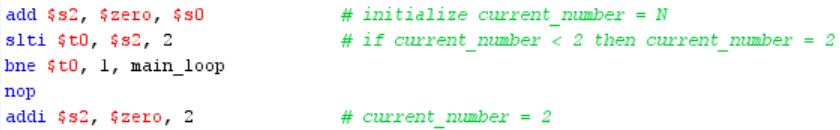
\includegraphics[scale=0.9]{5}
	\end{center}
	- Khối lệnh tiếp theo thực hiện khởi tạo giá trị cho biến \textit{current\_number} (Thanh ghi \$s2). Đầu tiên gán giá trị N cho \textit{current\_number}. Sau đó kiểm tra, nếu giá trị\\ \textit{current\_number} < 2 thì gán \textit{current\_number} = 2.
	\\- Thực hiện chương trình:\\
	Do giá trị N = 44 > 2 nên \textit{current\_number} = 2.
	\begin{center}
	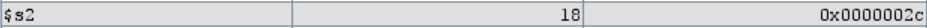
\includegraphics[scale=1]{6} 
	\end{center}
	\item Khối lệnh chính của chương trình: \textit{main\_loop}
	\begin{center}
	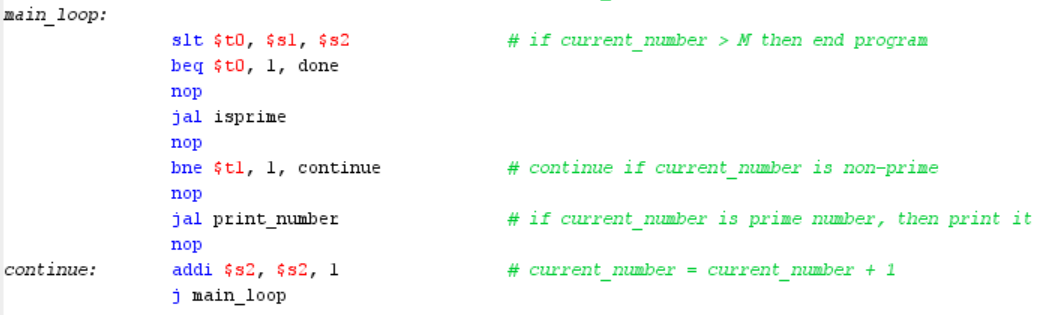
\includegraphics[scale=0.9]{7}
	\end{center}
	- Đầu tiên, chương trình sẽ kiểm tra nếu \textit{current\_number} > M thì sẽ kết thúc chương trình. 
	\\- Nếu \textit{current\_number} $\leq$ M thì chương trình sẽ gọi đến hàm \textit{isprime} \textit{(Chi tiết về hàm isprime ở phần sau)}. Hàm \textit{isprime} trả về giá trị nằm ở thanh ghi \$t1. Nếu \$t1 = 1 thì \textit{current\_number} là số nguyên tố, nếu \$t1 = 0 thì \textit{current\_number} không phải là số nguyên tố.
	\\- Nếu \$t1 = 1 thì chương trình sẽ gọi đến thủ tục \textit{print\_number} để thực hiện in giá trị \textit{current\_number} ra màn hình. 
	\\- \textit{Thực hiện chương trình:}
	\begin{itemize}
	\item[*] Giá trị hiện tại của \textit{current\_number} = 44. Thanh ghi \$t0 có giá trị = 0, vậy \\\textit{current\_number} $\leq$ M.
	\begin{center}
	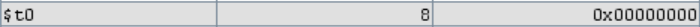
\includegraphics[scale=1]{8}
	\end{center}	 
	\item[*] Sau khi gọi đến hàm \textit{isprime}, thanh ghi \$pc nhảy đến địa chỉ của hàm \textit{isprime}, thanh ghi \$ra lưu giá trị của địa chỉ ngay sau lệnh \textit{jal} trong chương trình chính.
	\begin{center}
	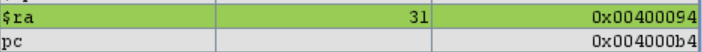
\includegraphics[scale=1]{9}
	\end{center}
	\pagebreak
	\item[*] Sau khi thực hiện xong hàm \textit{isprime}, do \textit{current\_number} = 44, không phải là số nguyên tố nên thanh ghi \$t1 = 0 và thanh ghi \$pc nhận giá trị mà thanh ghi \$ra đã cất giữ trước đó.
	\begin{center}
	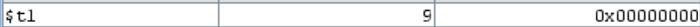
\includegraphics[scale=1]{11}
	\end{center}
	\begin{center}
	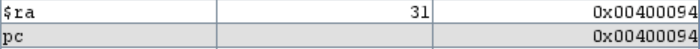
\includegraphics[scale=1]{10}
	\end{center}
	\end{itemize}
	\item Khối lệnh \textit{continue}
	\begin{center}
 	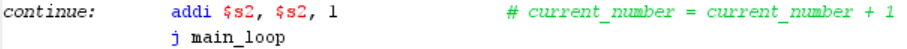
\includegraphics[scale=1]{12}
	\end{center}
	- Khối lệnh này thực hiện tăng giá trị \textit{current\_number} lên 1 đơn vị và quay lại nhãn \textit{main\_loop}.
\end{itemize}
\textbf{Kết quả thực hiện:}
\\Với input N = 44, M = 84
\begin{center}
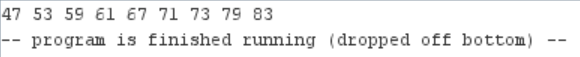
\includegraphics[scale=1]{18}
\end{center}
\pagebreak
\subsection*{Giải thích các thủ tục và hàm:}
\begin{itemize}
	\item Hàm \textit{isprime:}
	\\Hàm \textit{isprime} trả về giá trị nằm ở thanh ghi \$t1. Nếu \$t1 = 1 thì \textit{current\_number} là số nguyên tố, nếu \$t1 = 0 thì \textit{current\_number} không phải là số nguyên tố.
	\begin{itemize}
		\item Khối lệnh \textit{push}:
		\begin{center}
		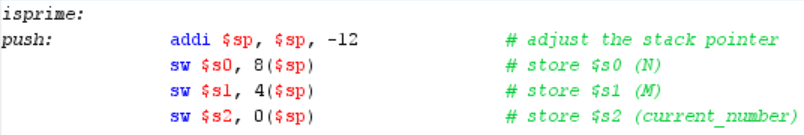
\includegraphics[scale=1]{13}
		\end{center}
		* Thực hiện lưu lại giá trị của 3 thanh ghi đầu vào (\$s0 - N, \$s1 - M, \$s2 - \textit{current\_number}) vào ngăn xếp để cất giữ.
		\item Khối lệnh \textit{work}:
		\begin{center}
		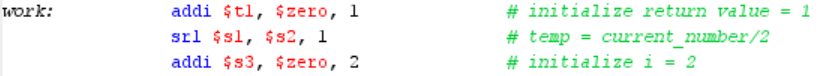
\includegraphics[scale=1]{14}
		\end{center}
		* Thực hiện khởi tạo 3 giá trị \$t1 = 1 (return number), \$s1 = \textit{current\_number}/2 (temp), \$s3 = 2 (i).
		\item Khối lệnh \textit{loop}:
		\begin{center}
		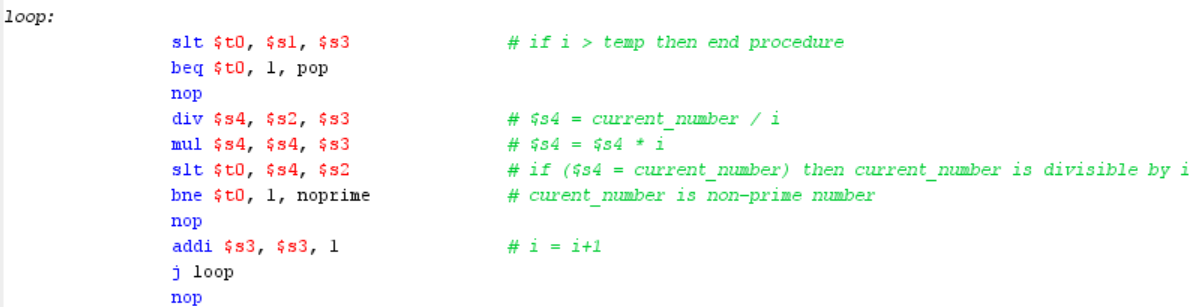
\includegraphics[scale=1]{15}
		\end{center}
		* Đầu tiên, chương trình sẽ kiểm tra nếu i > temp thì sẽ nhảy đến nhãn \textit{pop} để kết thúc hàm.\\
		* Thực hiện cho i chạy từ 2 -> \textit{current\_number}/2. Nếu \textit{current\_number} chia hết cho i thì chứng tỏ \textit{current\_number} không phải là số nguyên tố. \\
		* Tìm số dư của \textit{current\_number} / i bằng cách chia rồi lấy thương (giá trị nguyên) sau đó đem nhân lại với i. Nếu giá trị vừa nhân lên = \textit{current\_number} thì chứng tỏ \textit{current\_number} chia hết cho i, chương trình sẽ nhảy đến nhãn \textit{noprime}. Nếu \textit{current\_number} không chia hết cho i thì tăng i lên 1 đơn vị rồi quay lại nhãn \textit{loop}.
		\item Khối lệnh \textit{noprime} và \textit{pop}:
		\begin{center}
		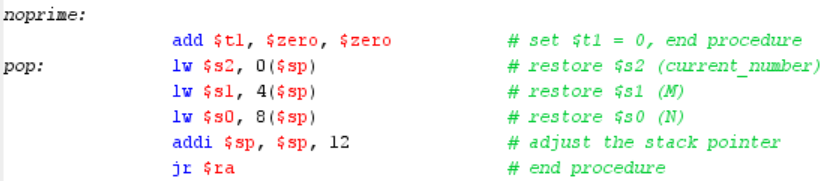
\includegraphics[scale=1]{16}
		\end{center}
		* Khối lệnh \textit{noprime} sẽ thực hiện gán giá trị trả về \$t1 = 0.\\	
		* Khối lệnh \textit{pop} thực hiện trả lại giá trị ban đầu cho các biến đã lưu trong ngăn xếp và giải phóng ngăn xếp, gọi lệnh \textit{jr} để quay về chương trình chính.
	\end{itemize}
	\item Hàm \textit{print\_number}
	\\Hàm \textit{print\_number in ra số nguyên tố được lưu ở thanh ghi \$s2}
	\begin{center}
	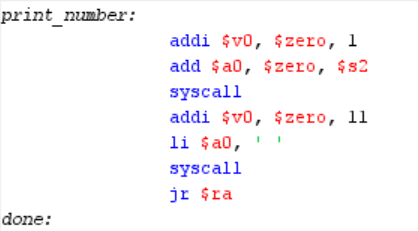
\includegraphics[scale=1]{17}
	\end{center}
	\begin{itemize}
	\item Đầu tiên, hàm sẽ gọi đến chức năng \textbf{print decimal integer} (\$v0 = 1) để in ra số nguyên tố được lưu trong thanh ghi \$s2.
	\item Sau đó, hàm sẽ gọi đến chức năng \textbf{print character} (\$v0 = 11) để in ra kí tự \textit{space}, giúp ngăn cách các số nguyên tố khi liệt kê.
	\end{itemize}
	

\end{itemize}
\end{document}